% The storage around one tube: half a section along the tube, from its axis outwards
\documentclass[tikz, border=4pt]{standalone}
% Shared preamble of the PyTES model diagrams: packages, colours and styles.
% Each diagram is a standalone document that inputs this file; build them with build.py.
\usepackage{amsmath}
\usepackage{bm}
\usetikzlibrary{arrows.meta, calc, decorations.pathreplacing, patterns, positioning}

% The PyTES Thermal colour cycle (pytes.plotting.THERMAL) and tints of it
\definecolor{pytesorange}{HTML}{E8590C}
\definecolor{pytesblue}{HTML}{1F4E9C}
\definecolor{pytesteal}{HTML}{14A08A}
\definecolor{pytesamber}{HTML}{F0A930}
\definecolor{pytesplum}{HTML}{A23B72}
\definecolor{pytessky}{HTML}{88C7F0}
\definecolor{pytesink}{HTML}{36312E}

% Materials: the heat transfer fluid, the PCM, the metal (fins and tubes)
\colorlet{fluidfill}{pytessky!75}
\colorlet{pcmfill}{pytesamber!55}
\colorlet{liquidfill}{pytesorange!60}
\colorlet{metalfill}{pytesink!45}
\colorlet{compositefill}{pcmfill!85!metalfill}

\tikzset{
  >={Stealth[length=2.2mm]},
  every picture/.style={line join=round, line cap=round, font=\small},
  outline/.style={draw=pytesink, line width=0.6pt},
  fluid/.style={outline, fill=fluidfill},
  pcm/.style={outline, fill=pcmfill},
  liquid/.style={outline, fill=liquidfill},
  metal/.style={outline, fill=metalfill},
  composite/.style={outline, fill=compositefill},
  flow/.style={->, draw=pytesblue, line width=1.2pt},
  heat/.style={->, draw=pytesorange, line width=1.1pt},
  axis/.style={->, draw=pytesink, line width=0.7pt},
  dimension/.style={<->, >={Stealth[length=1.6mm]}, draw=pytesink, line width=0.5pt},
  guide/.style={draw=pytesink!60, line width=0.4pt, dashed},
  symmetry/.style={draw=pytesink, line width=0.5pt, dash dot},
  label/.style={text=pytesink, font=\small},
  note/.style={text=pytesink, font=\footnotesize, align=center},
}

\begin{document}
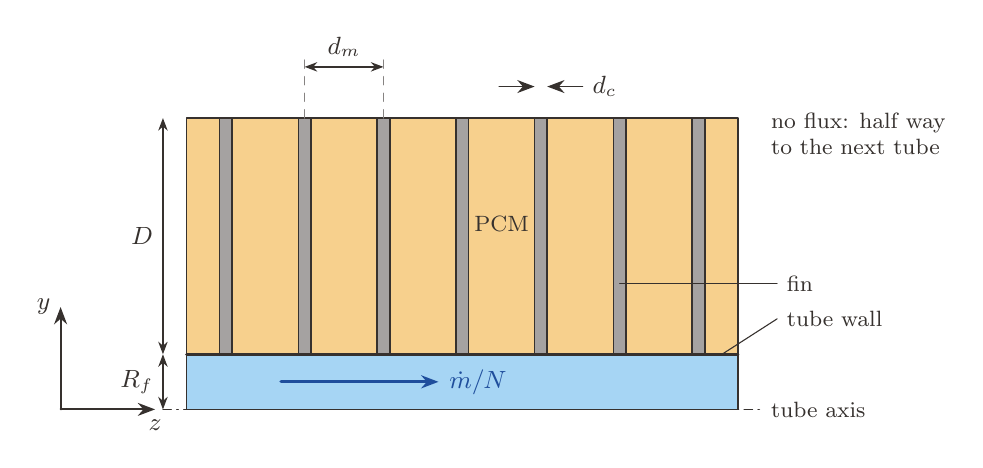
\begin{tikzpicture}
  \def\L{7.0}
  \def\Rf{0.7}
  \def\D{3.0}
  \def\dc{0.16}
  \def\dm{1.0}
  % Fluid in the tube, PCM, fins
  \draw[fluid] (0, 0) rectangle (\L, \Rf);
  \fill[pcmfill] (0, \Rf) rectangle (\L, \Rf + \D);
  \foreach \i in {0, ..., 6} {
    \draw[metal] ({0.5 + \i*\dm - \dc/2}, \Rf) rectangle ({0.5 + \i*\dm + \dc/2}, \Rf + \D);
  }
  \draw[outline] (0, \Rf) rectangle (\L, \Rf + \D);
  \draw[outline, line width=1.1pt] (0, \Rf) -- (\L, \Rf);
  \draw[symmetry] (-0.3, 0) -- (\L + 0.3, 0);
  \node[note, anchor=west] at (\L + 0.3, 0) {tube axis};
  \draw[flow] (1.2, \Rf/2) -- (3.2, \Rf/2) node[label, right, text=pytesblue] {$\dot m / N$};
  % Labels of the materials and the boundaries
  \node[note, fill=pcmfill, inner sep=1pt] at ({0.5 + 3.5*\dm}, \Rf + 0.55*\D) {PCM};
  \draw[pytesink, line width=0.4pt] ({0.5 + 5*\dm}, \Rf + 0.3*\D) -- (\L + 0.5, \Rf + 0.3*\D)
    node[note, anchor=west] {fin};
  \draw[pytesink, line width=0.4pt] (\L - 0.2, \Rf) -- (\L + 0.5, \Rf + 0.45)
    node[note, anchor=west] {tube wall};
  \node[note, anchor=west, align=left] at (\L + 0.3, \Rf + \D - 0.2)
    {no flux: half way\\to the next tube};
  % Coordinates and dimensions
  \draw[axis] (-1.6, 0) -- (-1.6, 1.3) node[label, left] {$y$};
  \draw[axis] (-1.6, 0) -- (-0.4, 0) node[label, below] {$z$};
  \draw[dimension] (-0.3, 0) -- (-0.3, \Rf) node[label, midway, left] {$R_f$};
  \draw[dimension] (-0.3, \Rf) -- (-0.3, \Rf + \D) node[label, midway, left] {$D$};
  \draw[dimension] ({0.5 + \dm}, \Rf + \D + 0.65) -- ({0.5 + 2*\dm}, \Rf + \D + 0.65)
    node[label, midway, above] {$d_m$};
  \draw[guide] ({0.5 + \dm}, \Rf + \D) -- ({0.5 + \dm}, \Rf + \D + 0.8);
  \draw[guide] ({0.5 + 2*\dm}, \Rf + \D) -- ({0.5 + 2*\dm}, \Rf + \D + 0.8);
  \draw[->, pytesink, line width=0.5pt] ({0.5 + 4*\dm - \dc/2 - 0.45}, \Rf + \D + 0.4)
    -- ({0.5 + 4*\dm - \dc/2}, \Rf + \D + 0.4);
  \draw[->, pytesink, line width=0.5pt] ({0.5 + 4*\dm + \dc/2 + 0.45}, \Rf + \D + 0.4)
    -- ({0.5 + 4*\dm + \dc/2}, \Rf + \D + 0.4) node[label, pos=0, right] {$d_c$};
\end{tikzpicture}
\end{document}
